\documentclass[11pt]{article}
\usepackage{neurips_2024}
\usepackage[UTF8,fontset=none]{ctex}
\setCJKmainfont{Hiragino Sans GB}
\setCJKsansfont{Hiragino Sans GB}
\setCJKmonofont{Hiragino Sans GB}
\usepackage{graphicx}
\usepackage{booktabs}
\usepackage{amsmath}
\usepackage{hyperref}
\usepackage{caption}
\usepackage{subcaption}
\usepackage{enumitem}
\setlist{nosep}

\title{基于 3DGS 与 AIGC 的多源资产生成与真实场景融合}
\author{深度学习与空间智能期末作业 Task 1}
\date{}

\begin{document}
\maketitle

\begin{abstract}
本项目完成了一个全链路 3D 视觉系统：首先使用 COLMAP 与 3D Gaussian Splatting (3DGS) 从真实多视角图像重建物体 A；随后分别使用 threestudio 的文本到 3D 生成和 Zero123 单图到 3D 生成得到物体 B 与物体 C；最后选择 Mip-NeRF 360 的 garden 场景作为背景，通过 3DGS 重建并将 ABC 三个资产插入同一世界坐标系，输出多视角环绕渲染视频。最终融合采用 ``garden + A'' 的显式高斯渲染与 B/C mesh 深度合成的混合表达方式，使生成资产和真实背景在相机环绕时保持相对静止。
\end{abstract}

\section{项目链接}
\textbf{GitHub:} \href{https://github.com/jiangjingshuang2-stack/Deep-Learning-Final}{github.com/jiangjingshuang2-stack/Deep-Learning-Final}。\\
\textbf{模型权重:} \href{https://drive.google.com/drive/folders/154-pIcfsTkYXpTeUgTcfOjBJ5Sep0xIy?dmr=1&ec=wgc-drive-%5Bmodule%5D-goto}{Google Drive 模型权重文件夹}。\\
\textbf{主要结果视频:} \texttt{videos/final\_ABC\_garden\_world\_static\_v2.mp4}。

\section{任务背景}
题目要求同时覆盖真实世界三维重建、AIGC 三维资产生成和真实场景融合渲染。3DGS 将场景表示为大量带颜色、不透明度、尺度和旋转的三维高斯，具有训练速度快、实时渲染质量高的优点；AIGC 资产通常以隐式场或 mesh 形式输出，和 3DGS 的显式高斯表达不同，因此最终融合的核心问题是坐标、尺度、表达形式和可见性关系的统一。

\section{数据集与资产}
\textbf{物体 A} 使用真实物体多视角图像。输入图像先顺时针旋转 90 度，再使用 COLMAP 完成特征提取、匹配和稀疏重建。经过 relaxed full-frame pinhole 设置后，得到 71 张有效相机位姿，并训练 3DGS 至 7000 iterations。

\textbf{物体 B} 使用 threestudio 的 DreamFusion/SDS 路径，仅输入文本 prompt：
\begin{quote}
\texttt{a small blue ceramic dragon statue, detailed scales, glossy surface, studio lighting}
\end{quote}
中文含义为：一个小型蓝色陶瓷龙雕像，具有细致的鳞片、光滑有光泽的表面，工作室灯光。

\textbf{物体 C} 使用单张去背景后的防晒霜图片，结合 Zero123 的新视角先验完成单图到 3D 生成。

\textbf{背景场景} 选择 Mip-NeRF 360 数据集中的 garden，并使用 3DGS 训练至 30000 iterations。

\section{方法}
\subsection{真实多视角物体 A 的 3DGS 重建}
首先使用 COLMAP 从多视角图像中恢复相机内外参和稀疏点云，再用 3DGS 优化每个高斯的均值、协方差、球谐颜色和透明度。训练目标为图像重建损失，主要由 L1 颜色项和结构相似性项组成：
\begin{equation}
\mathcal{L}=(1-\lambda)\mathcal{L}_{1}+\lambda \mathcal{L}_{D-SSIM}.
\end{equation}
为了增加有效位姿数量，使用了更宽松的匹配和 full-frame pinhole 相机设置。

\subsection{文本到 3D 物体 B}
物体 B 使用 SDS loss 将 2D 扩散模型的先验蒸馏到三维表示中。每次从当前三维表示随机渲染视角图像，再由扩散模型估计噪声残差并反向优化三维参数。该方法的优点是只需要文本，缺点是几何约束弱，细节和多视角一致性依赖扩散先验。

\subsection{单图到 3D 物体 C}
物体 C 使用 Zero123 从单张输入图像预测其他视角的一致外观，再在 threestudio 中优化出三维模型。与文本到 3D 相比，单图输入提供了更强的外观约束，因此纹理和主体类别更稳定，但背面和不可见区域仍依赖模型补全。

\subsection{背景 garden 的 3DGS 重建}
garden 场景直接使用开源多视角数据训练 3DGS。相比物体级重建，garden 的相机轨迹、遮挡和深度范围更复杂，但多视角覆盖充分，因此最终能提供稳定的真实环境背景。

\subsection{表达统一与最终融合}
本项目最终采用混合表达而不是简单贴图。garden 和 A 均为 3DGS，因此先将 A 的高斯点云进行过滤、尺度归一化、坐标变换，并插入 garden 的世界坐标系；B 和 C 从 threestudio 导出为带纹理 mesh，经过归一化、Z-up 到相机/世界坐标的转换后，固定到同一 garden 世界坐标中。渲染时先使用官方 3DGS renderer 输出 garden + A 帧，再使用同一相机轨迹对 B/C mesh 做深度合成。这样 ABC 与背景在环绕视频中保持世界静止关系。

\section{实验设置}
\begin{table}[H]
\centering
\caption{主要实验配置}
\begin{tabular}{lllll}
\toprule
资产 & 方法 & 训练步数 & 输入 & 输出表达 \\
\midrule
A & COLMAP + 3DGS & 7000 & 71 张有效多视角图像 & Gaussian PLY \\
B & DreamFusion / SDS & 5000 & 文本 prompt & textured mesh \\
C & Zero123 & 600 & 单张去背景图片 & textured mesh \\
garden & 3DGS & 30000 & Mip-NeRF 360 garden & Gaussian PLY \\
\bottomrule
\end{tabular}
\end{table}

\begin{table}[H]
\centering
\caption{超参数与日志信息}
\begin{tabular}{llll}
\toprule
项目 & Optimizer / Loss & 关键超参数 & 日志 \\
\midrule
A 3DGS & Adam, L1 + D-SSIM & iter=7000, GPU=2 & \texttt{objectA\_3dgs\_train\_7000.log} \\
B SDS & Adam, SDS loss & steps=5000, GPU=3 & W\&B run \texttt{7txhb0k5} \\
C Zero123 & Adam, Zero123 guidance & steps=600, GPU=0 & W\&B run \texttt{4azkmnu1} \\
garden 3DGS & Adam, L1 + D-SSIM & iter=30000, GPU=2 & \texttt{garden\_3dgs\_train\_30k...log} \\
\bottomrule
\end{tabular}
\end{table}

\begin{table}[H]
\centering
\caption{更详细的网络、训练与评价设置}
\begin{tabular}{llllll}
\toprule
项目 & Network Architecture & Batch Size & Learning Rate & Epochs/Steps & 评价指标 \\
\midrule
A & 3D Gaussian, SH color & 1 view/iter & 3DGS 默认调度 & 7000 iter & L1, PSNR \\
B & threestudio NeRF/mesh export & 1 view/iter & threestudio 默认 Adam & 5000 steps & SDS loss, 渲染检查 \\
C & Zero123 guidance + 3D field & 1 view/iter & threestudio 默认 Adam & 600 steps & guidance loss, 渲染检查 \\
garden & 3D Gaussian, SH color & 1 view/iter & 3DGS 默认调度 & 30000 iter & L1, PSNR \\
\bottomrule
\end{tabular}
\end{table}

\begin{table}[h]
\centering
\caption{关键评价指标}
\begin{tabular}{llll}
\toprule
项目 & Split & L1 $\downarrow$ & PSNR $\uparrow$ \\
\midrule
A 3DGS & test @ 7000 & 0.00943 & 25.97 \\
A 3DGS & train @ 7000 & 0.00478 & 31.81 \\
garden 3DGS & train @ 30000 & 0.02038 & 30.04 \\
C Zero123 & train @ 600 & 2.30 & -- \\
\bottomrule
\end{tabular}
\end{table}

\section{实验结果}
\begin{figure}[H]
\centering
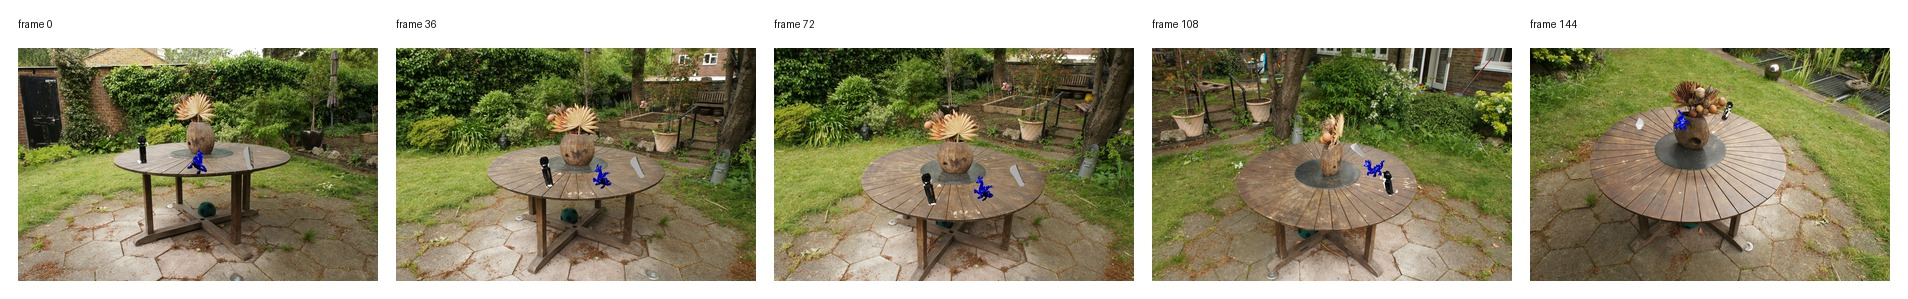
\includegraphics[width=\linewidth]{figures/fusion_world_static_v2_contact.jpg}
\caption{最终 v2 融合视频的多视角抽帧。ABC 与 garden 固定在同一世界坐标系中，相机环绕时物体与背景保持相对静止。}
\end{figure}

\begin{figure}[H]
\centering
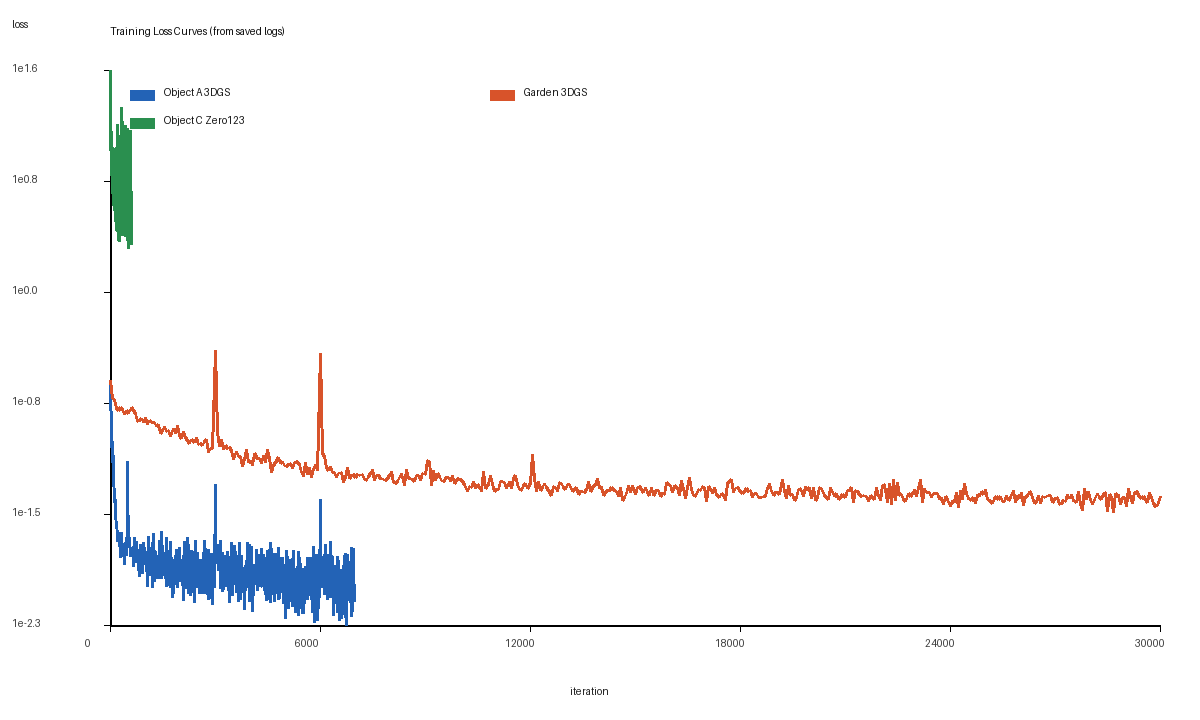
\includegraphics[width=0.85\linewidth]{figures/loss_curves_all.png}
\caption{由保存日志解析得到的训练曲线。B 的控制台日志未保存标量 loss，完整标量以 W\&B run 为准。}
\end{figure}

\begin{figure}[H]
\centering
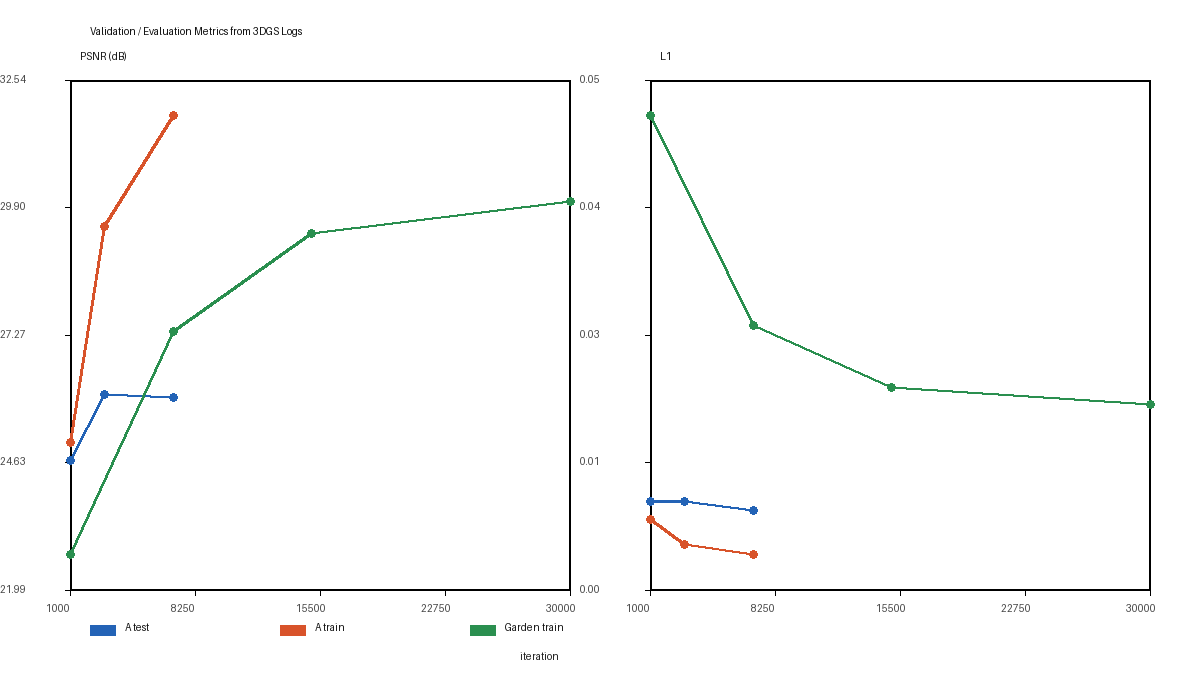
\includegraphics[width=0.85\linewidth]{figures/validation_metrics_3dgs.png}
\caption{验证/评价指标曲线。Object A 含 train/test 的 L1 与 PSNR，garden 日志记录 train L1 与 PSNR。B/C 的生成式资产主要以 W\&B 中的 guidance loss 与导出渲染进行检查。}
\end{figure}

\begin{figure}[H]
\centering
\begin{subfigure}{0.48\linewidth}
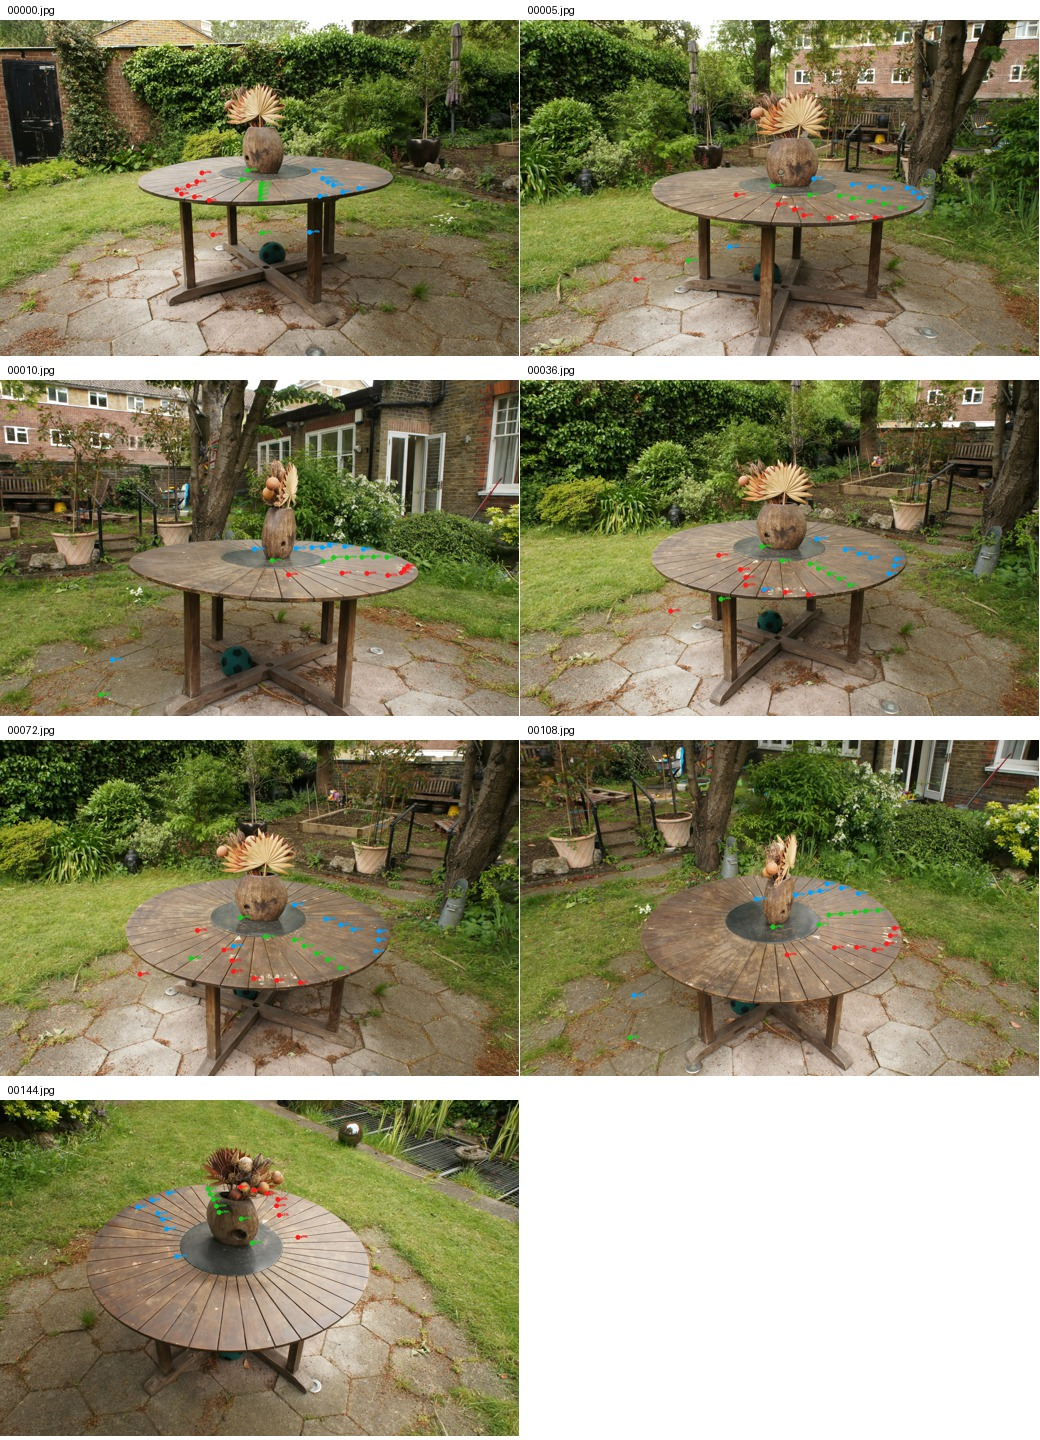
\includegraphics[width=\linewidth]{figures/table_candidates.jpg}
\caption{garden 桌面候选世界点}
\end{subfigure}
\begin{subfigure}{0.48\linewidth}
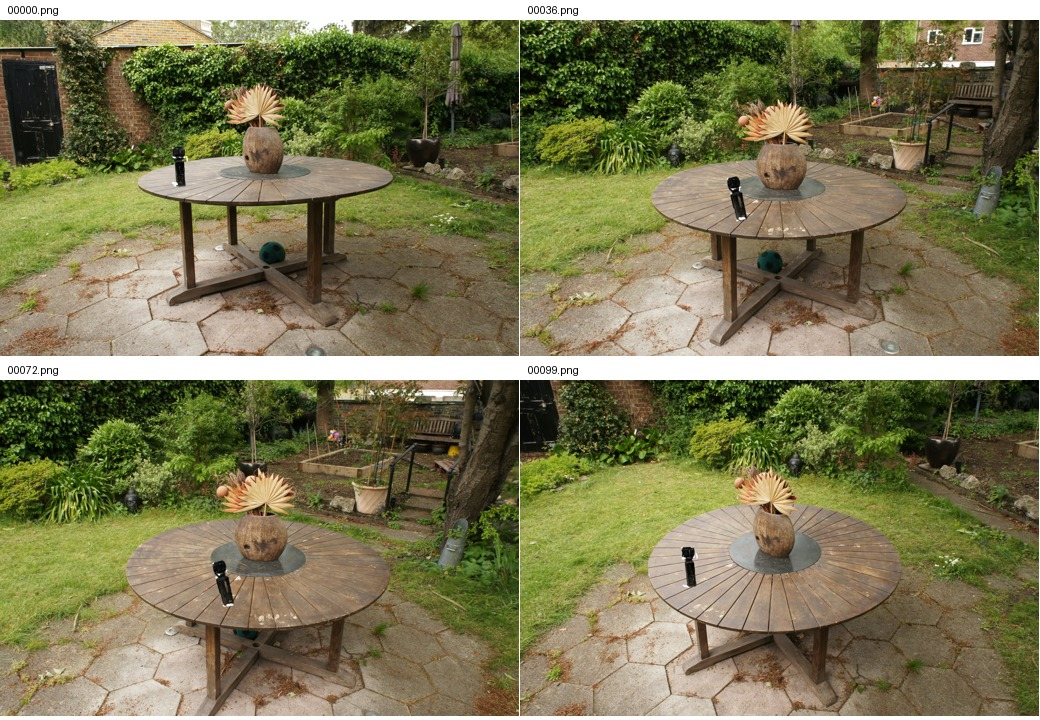
\includegraphics[width=\linewidth]{figures/a_v2_position_check.jpg}
\caption{A 在 v2 中上移后的检查}
\end{subfigure}
\caption{融合位置调试。最终 v2 将 A 略微上移，减少被桌面遮挡的问题。}
\end{figure}

\section{对比分析}
\begin{table}[H]
\centering
\caption{三种资产生成方式对比}
\begin{tabular}{llll}
\toprule
方式 & 几何准确度 & 纹理细节 & 计算耗时与稳定性 \\
\midrule
多视角重建 A & 最高，依赖 COLMAP 位姿 & 保留真实纹理，但受拍摄质量影响 & 位姿提取和 3DGS 训练成本中等 \\
文本生成 B & 类别和轮廓由扩散先验决定 & 风格化强，可能缺少真实细节 & 只需 prompt，但形状稳定性较弱 \\
单图生成 C & 正面准确，背面需补全 & 输入视角纹理较可靠 & 成本较低，受单图质量影响明显 \\
\bottomrule
\end{tabular}
\end{table}

从结果看，多视角重建最适合需要真实几何和真实纹理的资产；文本到 3D 更适合快速生成概念资产，但在本任务中 B 的龙形态在单独渲染时更明显，放入复杂背景后受尺度、视角和遮挡影响，识别性下降；单图到 3D 的 C 在正面纹理上最稳定，但背面几何不如多视角重建。

\section{现象与问题分析}
Object A 的主要难点是透明背景图像导致特征匹配不足，初始 COLMAP 只有较少有效位姿。通过放宽匹配和相机模型设置，有效位姿提升到 71 张。最终融合时 A 曾出现位置偏低，底部被 garden 桌面遮挡，因此 v2 版本沿相机上方向略微上移。

Object B 的问题主要来自生成模型与最终场景尺度的差异。单独渲染时相机围绕 B 旋转，龙形状更容易被观察；放入 garden 后，相机轨迹由背景决定，B 的局部细节在远景下变小，因此需要在最终融合中调整比例、朝向和位置。最终版本采用世界静止合成，避免了早期 ``屏幕贴片'' 式静态叠加的问题。

\section{结论}
本任务完成了从真实采集、AIGC 资产生成、背景重建到最终融合渲染的完整流程。最终交付包括四个单独渲染视频、一个 ABC+garden 世界静止融合视频、训练日志、融合代码和中英文 LaTeX 报告源码。实验表明，3DGS 对真实场景与真实物体重建具有较高保真度，而 AIGC 资产更依赖生成先验；在融合阶段，统一坐标系、尺度和可见性关系比单独资产质量更关键。

\end{document}
